\documentclass[11pt, oneside]{article}   	% use "amsart" instead of "article" for AMSLaTeX format
\usepackage{geometry}                		% See geometry.pdf to learn the layout options. There are lots.
\geometry{letterpaper}                   		% ... or a4paper or a5paper or ... 
%\geometry{landscape}                		% Activate for for rotated page geometry
%\usepackage[parfill]{parskip}    		% Activate to begin paragraphs with an empty line rather than an indent
\usepackage{graphicx}				% Use pdf, png, jpg, or eps� with pdflatex; use eps in DVI mode
								% TeX will automatically convert eps --> pdf in pdflatex		
\usepackage{amssymb}
\usepackage{amsmath}
\usepackage{parskip}

\title{Integration by parts}
%\author{The Author}
\date{}							% Activate to display a given date or no date
\graphicspath{{/Users/telliott_admin/Dropbox/Tex/png/}}

\begin{document}
\maketitle
%\section{}
%\subsection{}
\Large
Integration by parts comes from the product rule.
\[ (uv)' = v \ du +  u \ dv \]
The idea is that when we integrate this we will have
\[ \int (uv)' = uv = \int v \ du +  \int u \ dv  \]
Rearranging, we obtain
\[ \int u \ dv = uv - \int v \ du  \]
Just to be clear, with an explicit independent variable $x$ this is:
\[ \int u \frac{dv}{dx} \ dx = uv - \int v \frac{du}{dx} \ dx \]
\subsection*{examples}
As a first example, take 
\[ \int x \ e^x \ dx \]
If this were
\[ \int x \ e^{x^2} \ dx \]
there would be no problem, because upon differentiating $x^2$ using the chain rule, we will get the $x$ that we see in the example.  For the first problem, write
\[ u = x \]
\[ du = dx \]
\[ dv = e^x \ dx \]
this is what we have.  Now let's see how this simplifies things
\[ v = \int e^x \ dx = e^x \]
Using the formula
\[ \int u \ dv = uv - \int v \ du \]
\[ uv = xe^{x} \]
\[ \int v \ du = \int e^{x} \ dx = e^{x} \]
So
\[ \int x e^x \ dx =  xe^{x} - e^{x} \]
Check
\[ \frac{d}{dx} \ [ \ xe^{x} - e^{x}\ ]  = xe^{x}  \]
It is clear that the extra term in the answer is there to eliminate an extra term in the derivative.  This pattern is generally true with integration by parts.

Our old friend $\cos^2x$ can be solved by this method.
\[ \int \cos^2x \ dx \]
Let 
\[ u = \cos x \]
\[ du = -\sin x \ dx \]
\[ dv = \cos x \ dx \]
This is what we have.  Then
\[ v = \int \cos x \ dx = \sin x \]
Using the formula
\[ \int u \ dv = uv - \int v \ du \]
\[ uv = \sin x \ \cos x \]
\[ \int v \ du = \int -\sin^2 x \ dx = \int (\cos^2 x \ - 1) \  dx \]
which looks like no progress, but write out what we have
\[ \int \cos^2x \ dx = \sin x \ \cos x + x - \int \cos^2x dx \]
We put 2 of $\int \cos^2x$ on the left and then divide by 2 to give
\[ \int \cos^2x \ dx = \frac{1}{2} ( \sin x \ \cos x + x)\]
For an alternate form, recall that
\[ \sin x \ \cos x  = \frac{1}{2} \ \sin 2x \]
So this is just
\[ \frac{1}{2} \ [ \ \frac{1}{2} \ \sin 2x + x \ ] \]
\subsection*{more about $\cos^2 x$}
There are a few more things to be said about cosine squared.  First, recall the identity
\[ \sin^2 x + \cos^2 x = 1 \]
Integrate both sides
\[ \int \sin^2 x \ dx + \int \cos^2 x \ dx  = \int 1 \ dx = x \]
Then consider what these graphs look like

\begin{center}
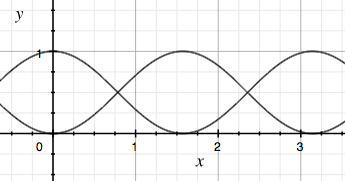
\includegraphics [scale=0.6] {sin2cos2.png}
\end{center}
Over the interval $x=0 \rightarrow \pi/2$ (or a multiple thereof), the area under the two curves is equal because they are mirror images, reflected about $\pi/4$.  
\[ \int_0^{\pi/2} \sin^2 x \ dx = \int_0^{\pi/2} \cos^2 x \ dx  \]

So, to obtain the area under a full lobe of the curve 
\[ \int_0^{\pi} \sin^2 x \ dx + \int_0^{\pi} \cos^2 x \ dx  = \int_0^{\pi} 1 \ dx = \pi \]
\[ \int_0^{\pi} \sin^2 x \ dx = \int_0^{\pi} \cos^2 x \ dx = \frac{\pi}{2} \]
which may be easier to remember than
\[ \int_0^{\pi} \cos^2x \ dx = \frac{1}{2} ( \sin x \ \cos x + x) \ \bigg |_0^{\pi} = \frac{1}{2} ( 0 + \pi - 0 - 0 ) =  \frac{\pi}{2} \]
It's interesting to compare this result with the area under the simple curves $\sin x$ and $\cos x$
\[ \int_0^{\pi} \sin x \ dx = - \cos x  \ \bigg |_0^{\pi} = -(-1 - 1) = 2 \]
The area under the sine or cosine is larger than the area under the square of either, because the values of sine and cosine are all less than one, so their squares are smaller than the values themselves.  The area under $f(x)$ from $f(x) = 0 \rightarrow f(x)=1$ is equal to $1$ for the sine or cosine, and to $\pi/4$ for the square.
\subsection*{back to integration by parts}
Now, consider 
\[ \int \ln x \ dx \]
It looks easy until you remember that you know the derivative, rather than the integral of $\ln(x)$.  So 
\[ u = \ln x \]
\[ du = \frac{1}{x} \ dx  \]
\[ dv = dx \]
Brilliant!  Then
\[ v = \int \ dx = x  \]
\[ \int u \ dv = uv - \int v \ du \]
\[ uv = x \ln x \]
\[ \int v \ du = \int x \ \frac{1}{x}  dx = x \]
We have
\[ \int \ln x \ dx = x \ \ln x - x \]
And again, when checking by differentiation, we see that the second term in the result is there to cancel one term from the product rule.

Here is one last elementary one.  Start by differentiating 
\[ \frac{d}{dx} \ x \sin x = x \cos x + \cos x \]
So, what will we do when faced with 
\[ \int x \cos x \ dx \]
Can you see that $x \sin x$ is the integral of $x \cos x$ except for the extra term?  If not, do this using our new method.
\[ u = x \]
\[ du = dx \]
\[ dv = \cos x \ dx \]
Then
\[ v = \int dv = \sin x \]
Using the formula
\[ \int u \ dv = uv - \int v \ du \]
\[ \int x \cos x \ dx = x \sin x - \int \sin x \ dx \]
\[ = x \sin x + \cos x \]

\subsection*{summary}
The way I think about this technique is I try to group the integral into terms that will be $dv$ and terms that will be $u$.  If $du$ is simpler than $u$, and if I can do the integral $\int dv = v$, then integration by parts is the way to go.  Here is a picture from Strang you may find illuminating

\begin{center}
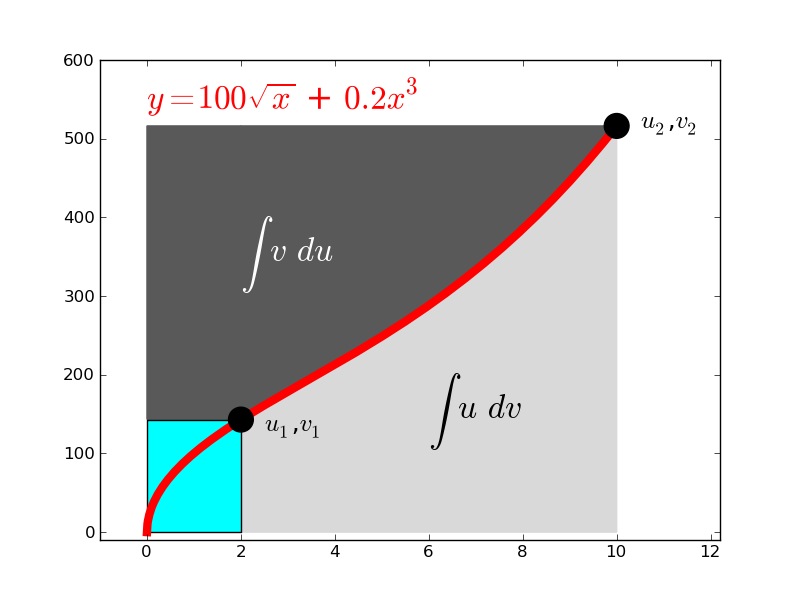
\includegraphics [scale=0.5] {ibp.png}
\end{center}

\subsection*{ocw problems}
I came across a video on MIT's ocw site giving four problems that are a little harder than what we've done above.  I thought I would work through them here.


Problem 1.
\[ \int x e^{-x} \ dx \]
We want to have the "u part" include stuff that will be easier after differentiation.  So
\[ u = x, \ \ du = dx \]
\[ dv = e^{-x} \ dx, \ \ v = -e^{-x} \]
\[ \int u \ dv = uv - \int v \ du \]
\[ uv = -xe^{-x} \]
\[ \int v \ du = \int -e^{-x} \ dx = e^{-x} \]
\[ \int x e^{-x} \ dx  =  -xe^{-x} - e^{-x} = -e^{-x}(1 + x) \]
Now
\[ \frac{d}{dx} -e^{-x}(1 + x) = -[ \ e^{-x} + (1 + x)(-e^{-x}) ] = xe^{-x}\]
So it checks.
\vspace{5 mm}

\noindent Problem 2.
\[ \int \frac{x^3}{(1+x^2)^2} \ dx \]
There's a trick here, which is to see that the $x^3$ should be split up, since one $x$ will serve as part of $dv$ to be integrated.
\[ u = x^2, \ \ du = 2 x \ dx \]
\[ dv = \frac{x}{(1+x^2)^2} \ dx, \ \ v = -\frac{1}{2}(\frac{1}{(1+x^2)} \]
so
\[ \int u \ dv = uv - \int v \ du \]
\[ uv = -\frac{x^2}{2}(\frac{1}{(1+x^2)} \]
\[ \int v \ du = -\frac{1}{2}(\frac{1}{(1+x^2)} \ 2x \ dx = - \int \frac{x}{(1+x^2)} \ dx = - \frac{1}{2} \ [ \ ln(1+x^2) \ ] \]
\[ \int \frac{x^3}{(1+x^2)^2} \ dx = -\frac{x^2}{2}(\frac{1}{(1+x^2)}) + \frac{1}{2} \ [ \ ln(1+x^2) =  \frac{1}{2}[ln(1+x^2) - \frac{x^2}{(1+x^2)} ]\]
Now
\[ \frac{d}{dx} [ \ \frac{1}{2}[ln(1+x^2) - \frac{x^2}{(1+x^2)}] = \ ?? \]
Let's do one piece at a time
\[ \frac{d}{dx} ln(1+x^2) = \frac{2x}{(1+x^2)} \]
\[ \frac{d}{dx} \frac{x^2}{(1+x^2)} = \frac{(1+x^2)2x - x^2(2x)}{(1+x^2)^2} =\frac{2x}{(1+x^2)} -  \frac{2x^3}{(1+x^2)^2} \]
Notice the minus sign between the two terms we are differentiating, that means we can cancel the terms $2x/(1+x)^2$ and switch the sign of the $x^3$ term, and then have
\[ \frac{1}{2} \frac{2x^3}{(1+x^2)^2} = \frac{x^3}{(1+x^2)^2} \]
So it checks.
\vspace{5 mm}

\noindent Problem 3.
\[ \int \frac{\ln x}{x^2} \ dx \]
We can integrate $\ln x$ (see above).  But usually, simplification comes by going in the opposite direction, so put it in $u$
\[ u = \ln x, \ \ du = \frac{1}{x} \ dx \]
\[ dv = \frac{1}{x^2} \ dx, \ \ v = -x^{-1} = -\frac{1}{x} \]
\[ \int u \ dv = uv - \int v \ du \]
\[ uv = -\frac{1}{x} \ln x\]
\[ \int v \ du = \int -\frac{1}{x^2} \ dx = \frac{1}{x} \]
\[ \int \frac{\ln x}{x^2} \ dx = -\frac{1}{x} \ln x - \frac{1}{x} = -\frac{1}{x}(1 + \ln x) \]
Now
\[ \frac{d}{dx} [ \ -\frac{1}{x}(1 + \ln x) \ ] = -\frac{1}{x^2} + \frac{(1 + \ln x)}{x^2} = \frac{\ln x}{x^2} \]
So it checks.
\vspace{5 mm}

\noindent Problem 4.
\[ \int \arctan \ x \ dx \]
It doesn't look like we have two terms here.  But we do..
\[ u = \arctan \ x, \ \ du =  \frac{1}{(1+x^2)} \ dx \]
\[ dv = 1 \ dx, \ \ v = x \]
\[ \int u \ dv = uv - \int v \ du \]
\[ uv = x \arctan \ x \]
\[ \int v \ du = \int  \frac{x}{(1+x^2)} \ dx = \frac{1}{2} \ln (1+x^2) \]
\[ \int \arctan \ x \ dx = x \arctan \ x - \frac{1}{2} \ln (1+x^2) \]
Now
\[ \frac{d}{dx} [ \ x \arctan \ x - \frac{1}{2} \ln (1+x^2) = ?? \]
The first term is
\[ \frac{x}{(1+x^2)} + \arctan \ x \]
and the second is
\[ - \frac{x}{(1+x^2)} \]
So it checks.
\vspace{5 mm}

\noindent Last problem.
\[ \int p^3 e^{-p^2} \ dp \]
\[ u = p^2, \ \ du =  2p \ dp \]
\[ dv = pe^{-p^2}, \ \ v = -\frac{1}{2} \ e^{-p^2} \]
\[ \int u \ dv = uv - \int v \ du \]
\[ uv = -\frac{1}{2} \ p^2 e^{-p^2} \]
\[ \int v \ du = \int -\frac{1}{2} \ e^{-p^2} \ 2p \ dp = -\int p \ e^{-p^2} \ dp = \frac{1}{2} \ e^{-p^2} \]
\[ \int p^3 e^{-p^2} \ dp = -\frac{1}{2} \ p^2 e^{-p^2} - \frac{1}{2} \ e^{-p^2} =  -\frac{1}{2} \ e^{-p^2}(1 + p^2)\]
I also did this a different way, with a double substitution, same answer.
\[ \int p^3 e^{-p^2} \ dp \]
\[ x = e^{-p^2}, \ \ dx =  -2p e^{-p^2} \ dp, \ \ -p^2 = \ln x \ !! \]
\[ \int p^3 e^{-p^2} \ dp = \frac{1}{2} \int \ln x \ dx \]
This one is integration by parts too, but perhaps we can just guess
\[ \frac{d}{dx} (x\ln x - x) = x \frac{1}{x} + \ln x - 1 = \ln x \]
Pick up the factor of $1/2$
\[ \frac{1}{2} \ ( x \ln x - x) = \frac{1}{2} \ [\ (-e^{-p^2}p^2) - e^{-p^2} \ ] \ = -\frac{1}{2} \ e^{-p^2}(1  + p^2) \] 
which is just what we had before.

\subsection*{one more example}
\[ \int e^x \cos x \ dx \]
Let
\[ u = e^x, \ \ \ du = e^x \ dx \]
\[ dv = \cos x  \ dx, \ \ \ v = \sin x \]
Then the integral is $uv - \int v \ du$ or
\[ = e^x \sin x - \int e^x \sin x \ dx \]
which looks like no help, but keep going.  Lather, rinse, repeat:
\[ u = e^x, \ \ \ du = e^x \ dx \]
\[ dv = - \sin x \ dx, \ \ \ v = \cos x \]
Then the second integral is
\[ - \int e^x \sin x \ dx = e^x \cos x - \int e^x \cos x \ dx \]
Putting the answers together:
\[ \int e^x \cos x \ dx = e^x \sin x + e^x \cos x - \int e^x \cos x \ dx \]
so
\[ 2 \int e^x \cos x \ dx = e^x \sin x + e^x \cos x \]
\[ \int e^x \cos x \ dx = \frac{1}{2} \ e^x \ [ \ \sin x + \cos x \ ] \]
Check by differentiating.  Leave the factor of $1/2$ aside for the moment:
\[ \frac{d}{dx} \ e^x \ [ \ \sin x + \cos x \ ] \ = e^x \ [ \ \sin x + \cos x \ ] + e^x \ [  \ \cos x - \sin x \ ] \]
The $\sin x$ terms cancel, giving $2$ terms of $\cos x$ but we have the factor of $1/2$ so that finally gives:
\[ \frac{d}{dx} \ e^x \ [ \ \sin x + \cos x \ ] \ = e^x \cos x  \]


\end{document}  